\documentclass{mc2015}

%%%%%%%%%%%%%%%%%%%%%%%%%%%%%%%%%%%%%%%%%%%%%%%%%%%%%%%%%%%%%%%%%%%%%
\usepackage[T1]{fontenc}         % Use T1 encoding instead of OT1
\usepackage[utf8]{inputenc}      % Use UTF8 input encoding
\usepackage{microtype}           % Improve typography
\usepackage{booktabs}            % Publication quality tables
\usepackage{amsmath}
\usepackage{graphicx}
\usepackage{float}
\usepackage[exponent-product=\cdot]{siunitx}
\usepackage[colorlinks,breaklinks]{hyperref}
\hypersetup{linkcolor=black, citecolor=black, urlcolor=black}

\usepackage{lipsum}

\def\equationautorefname{Eq.}
\def\figureautorefname{Fig.}

%%%%%%%%%%%%%%%%%%%%%%%%%%%%%%%%%%%%%%%%%%%%%%%%%%%%%%%%%%%%%%%%%%%%%
% Insert authors' names and short version of title in lines below

\authorHead{Chris Dances, Vince Mousseau, Maria Avramova}
\shortTitle{Initial Verification of CTF}

%%%%%%%%%%%%%%%%%%%%%%%%%%%%%%%%%%%%%%%%%%%%%%%%%%%%%%%%%%%%%%%%%%%%%
\begin{document}

\title{Initial 1-D Single Phase Liquid Verification of CTF}

\author{Chris Dances}
\author{Dr. Maria Avramova}
\affil{ Department of Mechanical and Nuclear Engineering \\
  The Pennsylvania State University \\
  137 Reber Building, University Park, PA, 16802, USA \\
  cad39@psu.edu; mna109@psu.edu}

\author{Dr. Vince Mousseau}
\affil{ Computer Science Research Institute \\
  Sandia National Laboratories \\
  1450 Innovation Parkway, Albuquerque, NM 87123, USA \\
  vamouss@sandia.gov
}

\maketitle

\begin{abstract}
Nuclear engineering codes are being used to simulate more challenging problems
and at higher fidelities than they were initially developed for. In order to
expand the capabilities of these codes, state of the art numerical methods and
computer science need to be implemented. One of the key players in this effort
is the Consortium for Advanced Simulation of Light Water Reactors (CASL) through
development of the Virtual Environment for Reactor Applications (VERA). The
sub-channel thermal hydraulic code used in VERA, COBRA-TF (Coolant-Boiling in
Rod Arrays - Three Fluids), is partially developed at the Pennsylvania State
University by the Reactor Dynamics and Fuel Management Research Group (RDFMG).
The RDFMG of version COBRA-TF is referred to as CTF.

In an effort to help meet the objectives of CASL, a version of CTF has been
developed that solves the residual formulation of the one dimensional 
single-phase conservation equations. The formulation of the base equations as
residuals allows the for the isoloation of different sources of error and is a
good tool for verification purposes. This paper outlines the initial
verification work of both the original version of CTF and its residual
formulation. The verification problem is a simple 1-D single phase liquid
channel with no heat conduction, friction, and gravity. A transient boundary
condition is applied that alters the inlet density and temperature while keeping
the velocity within the channel constant. The constant velocity simplifies the modified
equation analysis and the order of accuracy is readily obtained. A Richardson
extrapolation is performed on the problem on the temporal and spatial step sizes
to determine the convergence and order of accuracy of the discretization error.
While extensive validation work has been present for CTF, there has been little
to no verification work previously. 

\emph{Key Words}: CTF, thermal hydraulic, verifiation, residual, Richardson
extrapolation, CASL

\end{abstract}

\clearpage
%%%%%%%%%%%%%%%%%%%%%%%%%%%%%%%%%%%%%%%%%%%%%%%%%%%%%%%%%%%%%%%%%%%%%

%\tableofcontents
%\clearpage
%
%\listoffigures
%\clearpage

%%%%%%%%%%%%%%%%%%%%%%%%%%%%%%%%%%%%%%%%%%%%%%%%%%%%%%%%%%%%%%%%%%%%%
\section{Introduction}

For the past several decades, the primary focus in nuclear engineering within
the United States has been focused on light water reactors (LWR). Commercially,
all nuclear reactors are either boiling water reactors (BWR) or pressurized
water reactors (PWR). Correct computation of the thermal hydraulics within the
reactor core leads to efficient design and accuracy in the safety analysis. A
popular subchannel code for modelling the hydrodynamics within the reactor core
is CTF. This FORTRAN based code solves 8 conservation equations for liquid,
entrained droplet, and vapor phases in 3-D dimensions \cite{CTF_Theory}. A 1-D
residual formulation of the code has been created. This paper outlines an
initial verification of the original version of code as well as the residual
version of the code. The verification problem is a single phase 1-D channel with
transient inlet density and mass flow rate. The problem will undergo a
Richardson's extrapolation in the temporal and spatial domains to verify the
convergence and order of accuracy of the error. The study of the order of
accuracy is considered one of the more rigorous verification criteria
\cite{VV_review}.

\section{CTF}

The thermal hydraulics of a LWR core is an important part of nuclear
reactor design. CTF solves 8 conservation equations for liquid,
entrained droplet, and vapor phases of water boiling within the rod structure
of a LWR reactor core \cite{CTF_Theory}. Currently, the conservation
equations analytically reduce into a pressure matrix in a semi-implicit
method with rod temperatures solved for explicitly. The residual formulation of
the code currently solves the 1-D single phase liquid conservation equations and
calculated variables in a residual formulation. While it has the ability to
solve the code semi-implicitly or implicitly, only the semi-implicit
solution method is considered in this paper. This residual formulation should
allow for easier and more in depth verification  analysis. This paper details
the initial comparison of the residual  formulation to the original code.

\subsection{Software Quality Assurance}

Software quality assurance is a set of tools and procedures that helps
ensure that the software is reliable. CTF is managed by GitHub repository
setup and maintained by CASL. An extensive test matrix is run before each major
push to ensure that the code meets the specified requirements. The test matrix
consists of unit tests, code coverage runs, validation problems, and challenge
problems. The code documentation consists of a theory manual, a user manual, a
developer manual, and a validation manual. Further work might involve using
auto documentation tools to keep an up to date developers manual. This paper
will be the beginning of a verification manual, integrating this verification
problem directly into the test matrix.

\subsection{1-D Single Phase Liquid Conservation Equations}

The finite volume structure in CTF in figure \ref{fig:CTF-Cells} is for a
one-dimensional channel in the axial direction with $n$ number of cells. The
first and last cells at 0 and $n+1$ are ghost cells and act as the boundary
conditions for the problem. Pressure, enthalpy, and density are averaged over
the cell volume and are located at the center of the cell. Mass flow rate and
velocity are located at the faces in between cells. The cells  are represented
with an index $i$, and the faces with indexes of $i + \frac{1}{2}$ or 
$i-\frac{1}{2}$. This project will initially focus on this 1-D configuration.
Usually the code  is 3-D,  with channels connecting to each other in two more 
dimensions.

\begin{figure}[!h]
	\centering
	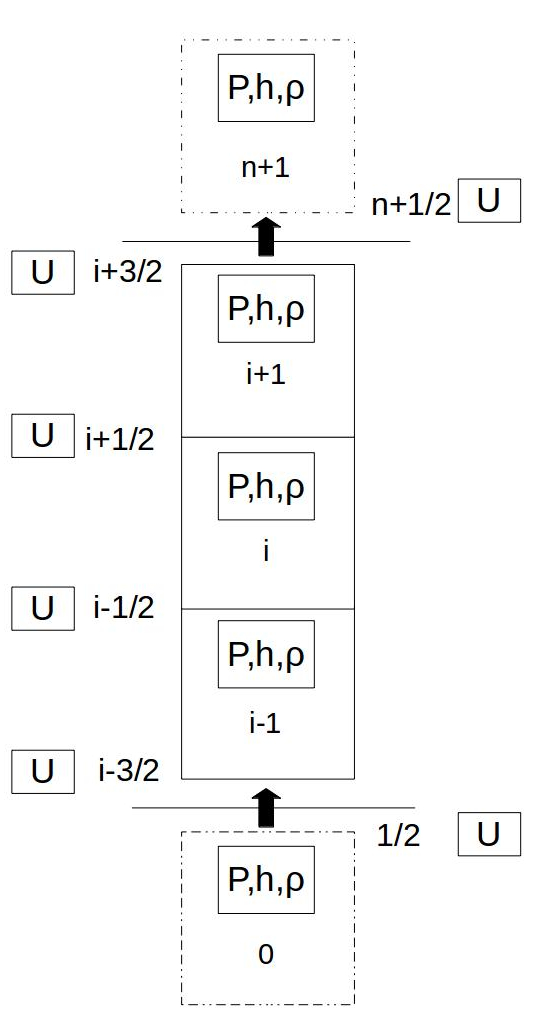
\includegraphics[width=0.30\textwidth]{images/CTF-Cells}
	\caption{The finite volume structure for CTF}
	\label{fig:CTF-Cells}
\end{figure}

The single phase Euler partial differential equations for mass
\eqref{eq:pde_mass}, momentum \eqref{eq:pde_momentum}, and energy
\eqref{eq:pde_energy} correspond to the unknown variables pressure $P$,
velocity $u$, and enthalpy $h$. Density $\rho$ is related through the equation
of state. The first terms in each of the equations are temporal terms. The rest
of the terms are steady state spatial terms. 
    
    \begin{equation}
    	\label{eq:pde_mass}
    	\frac{ \partial \rho}{\partial t} + \bigtriangledown \rho u = 0
    \end{equation}
    
    \begin{equation}
    	\label{eq:pde_momentum}
    	\frac{ \partial \rho u}{\partial t} + \bigtriangledown \rho u^{2} +
    	\bigtriangledown P - \rho g  = 0
    \end{equation}
    
    \begin{equation}
    	\label{eq:pde_energy}
    	\frac{ \partial \rho h}{\partial t} -
    	\frac{ \partial  P}{\partial t} + 
    	\bigtriangledown ( \rho  u h )
    	= 0
    \end{equation}

\subsection{Residual Formulation and Jacobian Construction}

	A residual is simply the difference between the value at some future time
    $n+1$ and the value at the current iteration $k$. This can be applied to
    desired variables and equations. For example, the residual for density,
    $\delta \rho_{i}$, is the difference between iterate levels
    $n+1$ and $k$, $\rho^{n+1}_{i} - \rho^{k}_{i}$. The residuals for the
    equations are determined by substituting the residuals into the discretized
    equations, which should effectively change all $n+1$ into $k$. Each cell
    will have three residual variables and three residual equations. For the
    entire solution, we will then have a residual variable array $\delta X$, and
    a residual function array $F(X)$ which defines a linear system $J \delta X =
    - F(X)$.
    
    The Jacobian matrix is defined as the derivative
    of each response of the function $F_{j}$ with respect to each variable $X_{i}$.
    The derivative can be calculated numerically as shown by equation
    \eqref{eq:jac_numerical} where $\epsilon$ is a small numerical value. For
    CTF the equations are linear, and this numerical approximation
    of the Jacobian matrix is exact. This should produce the same Jacobian
    matrix that CTF currently generates analytically. 
    
    \begin{equation}
    	\label{eq:jac_numerical}
    	J_{i,j}=\frac{ \partial F_{j}(X)}{\partial X_{i}}
    	      \approx \frac{F_{j}(X_{i}+\epsilon)-F_{j}(X)}{\epsilon}
    \end{equation}
    
	To build the Jacobian matrix, an object oriented class was created that
    contains three arrays. An array that points to the residual functions, an
    array that points to the position within a target variable array, and an
    array that has the index that the function is to be evaluated at. These
    lists can be appended in any order, but they have to be appended
    simultaneously such that variables and functions correspond with each
    other. Then to construct the Jacobian matrix, the residual function and
    residual variable arrays can each be looped over to numerically build the
    Jacobian matrix as seen in figure \ref{fig:Jacobian_Setup}. 
    
    \begin{figure}[!h]
    	\centering
    	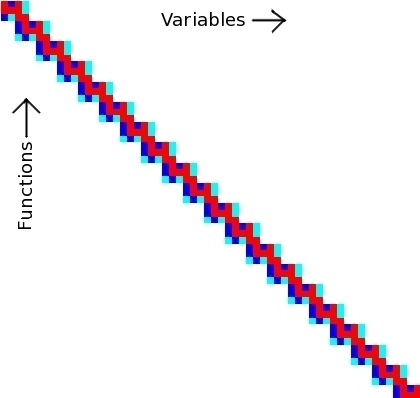
\includegraphics[width=0.40\textwidth]{images/Jacobian_Setup}
    	\caption{Structure of the Jacobian matrix for single phase liquid}
    	\label{fig:Jacobian_Setup}
    \end{figure}

\section{Isokinetic Sine Wave Advection}

Code verification is the set of procedures set in place to ensure that the code
was written properly. The procedures can use the following as code verification
criteria from least to most rigorous are expert judgement, error quantification,
consistency / convergence, and order of accuracy \cite{VV_Book}. For this work,
the Richardson Extrapolation will be used to check for convergence and order
of accuracy of the error in space and time. The error should converge to zero,
and the order of accuracy should converge to the values obtained through the
modified equation analysis at the end of this section.
 
\subsection{Problem Setup}

%Round off error, iterative convergence error.
%Discretization error?? (Check with)

The verification problem is defined as a single horizontal channel with
base parameters listed in table \ref{table:parameters}. Channel area and
perimeter are constant across the entire height of the channel. No grid spacers
are present, and frictional losses are set to zero. Velocity and pressure
are assumed to be constant, but small fluctuations may occur due to coding
mistakes or numerical roundoff. The channel geometry and
operating conditions approximate a standard PWR. The inlet of the channel has a
constant velocity with a fluctuating enthalpy that corresponds to a 37.5
$^\circ$C temperature change.  The length of the transient was defined to be
quadruple the time needed for the liquid at the inlet to advect to the
outlet.The frequency of the sine wave was defined to generate a full period of a
spatial wave across the height of the channel.

\begin{table}[h]
\center
\caption{Problem Parameters}
\label{table:parameters}
\begin{tabular}{|c|c|c|c|}
\hline
Parameter	&	Symbol	&	Value	&	Unit	\\ \hline
Axial Height	&	$H$	&	3.6586	&	$m$	\\ \hline
Channel Area	&	$A_{ch}$	&	4.94E-005	&	$m^{2}$	\\ \hline
Wetted Perimeter	&	$P_{w}$	&	1.49E-002	&	$m$	\\ \hline
Velocity	&	$V_{o}$	&	7.35	&	$\frac{m}{s}$	\\ \hline
Pressure	&	$P_{o}$	&	155.00	&	bar	\\ \hline
Temperature 1	&	$T_{1}$	&	289.500	&	$^{\circ}$C	\\ \hline
Temperature 2	&	$T_{2}$	&	327.00	&	$^{\circ}$C	\\ \hline
Enthalpy 1	&	$h_{1}$	&	1281.55	&	$\frac{kJ}{kg}$	\\ \hline
Enthalpy 2	&	$h_{2}$	&	1497.21	&	$\frac{kJ}{kg}$	\\ \hline
Mass Flow Rate 1	&	$\dot{m}_{1}$	&	0.2713	&	$\frac{kg}{s}$	\\ \hline
Mass Flow Rate 2	&	$\dot{m}_{2}$	&	0.2399	&	$\frac{kg}{s}$	\\ \hline
Final Time	&	$t_{f}$	&	2.00	&	sec	\\ \hline
Wave Frequency	&	$\omega$	&	1.00	&	Hz	\\ \hline
\end{tabular}
\end{table}

The lookup table to vary the inlet enthalpy $h$ and inlet mass
flow rate, $\dot{m}$, are genererated from equations \ref{eq:Sine_Wave:h} and
\ref{eq:Sine_Wave:m_dot} respectively. The trignometric functions assume
constant axial spacing, $\Delta x$, and time step size, $\Delta t$, where $i$
and $j$ are the spatial and temporal indices. These equations should also
behave as the known solutions throughout the entire domain of the problem. The
enthalpy and mass flow rate vary proportionally to the density such that an
isokinetic boundary condition is created at the inlet. However, this is
dependent on the steam tables used in generating the input and calculating the
EOS. A python script was used to generate the data tables according to
trignometric equations using lookup tables that mimic the IAPWS-97 steam tables
used by the code \cite{IAPWS}.

\begin{equation}
	\label{eq:Sine_Wave:h}
	h(i,j) = \frac{1}{2} \left( 
			(h_{1}+h_{2}) + (h_{1}-h_{2}) cos\left(
				\omega \left( j \Delta t + \frac{i \Delta x}{V_{o}} \right)
				\right)
			\right)
\end{equation}

\begin{equation}
	\label{eq:Sine_Wave:m_dot}
	\dot{m}(i,j) = \frac{1}{2} \left( 
			(\dot{m}_{1}+\dot{m}_{2}) + (\dot{m}_{1}-\dot{m}_{2}) cos\left(
				\omega \left( j \Delta t + \frac{i \Delta x}{V_{o}} \right)
				\right)
			\right)
\end{equation}


The comparison between the data table and the output in CTF are shown for
enthalpy and mass flow rate in figures \ref{fig:Inlet_h} and
\ref{fig:Inlet_m_dot}, respectively. The CTF output was read from hdf5 data
files at each point in time, which omitted the actual ghost cell where these values
were applied. The CTF values are located at the nearest node to the inlet, and
will be slightly out of phase to the exact values. For large mesh sizes this
small discrepancy is not noticeable.

\begin{figure}[!h]
	\centering
	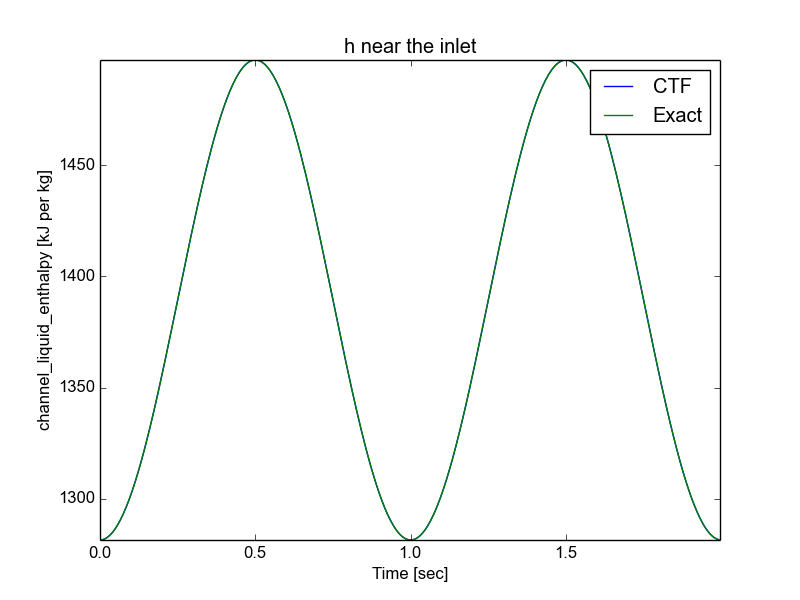
\includegraphics[width=0.55\textwidth]{images/Code_Verification/run_00_00/residual/results/Inlet_h}
	\caption{Enthalpy Near the Inlet and the Analytical Solution}
	\label{fig:Inlet_h}
\end{figure}

\begin{figure}[!h]
	\centering
	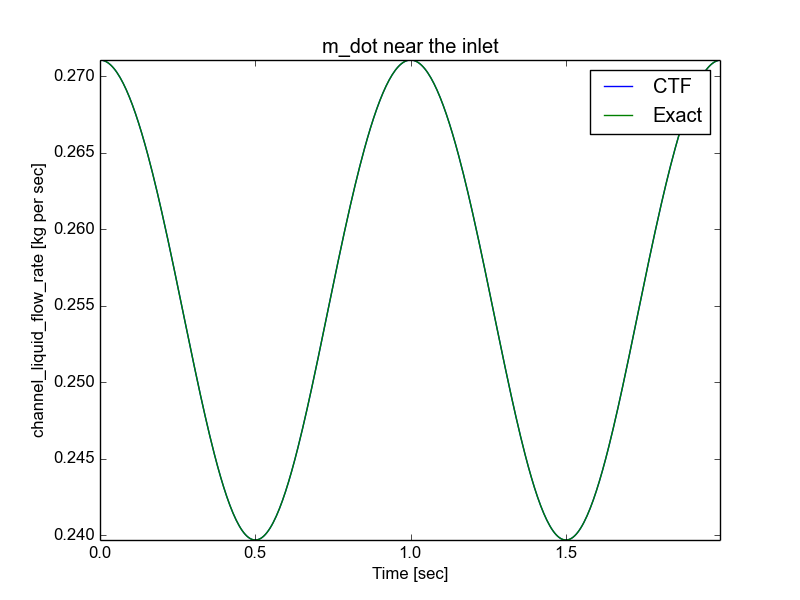
\includegraphics[width=0.55\textwidth]{images/Code_Verification/run_00_00/residual/results/Inlet_m_dot}
	\caption{Density Near the Inlet and the Analytical Solution}
	\label{fig:Inlet_m_dot}
\end{figure}

 For the original version of CTF, there is a small discrepancy in the way the
 density is calculated at the inlet that causes the velocity to be non-constant.
%as shown in figure \ref{fig:Inlet_vel}.
 This is considered small for this problem and should not greatly affect the
 order of accuracy. The residual formulation was coded in such a way as to avoid
 this problem and has considerably less fluctuation in the inlet velocity. The
 hdf5 output files allow for a high level of precision, reducing
 round off error in the output. 

\subsection{Code Convergence}

The current version of CTF uses global code convergence criteria that are
used to estimate the error associated with the solution of the code for
transient and steady state problems. The transient values of these criteria are
shown in figure \ref{fig:Code_Convergence:Original} for the original version of
CTF simulating the verification problem. The mass terms are in units of
$\frac{kg}{s}$, and the energy terms in units of $kW$. The solid energy storage
is zero since there are not any heat structures present. The fluctuating values
represent differences between the energy and mass entering and leaving the
system. The flat profile for the mass storage term means that the sine wave has
fully developed spatially through the channel. 

\begin{figure}[!h]
	\centering
	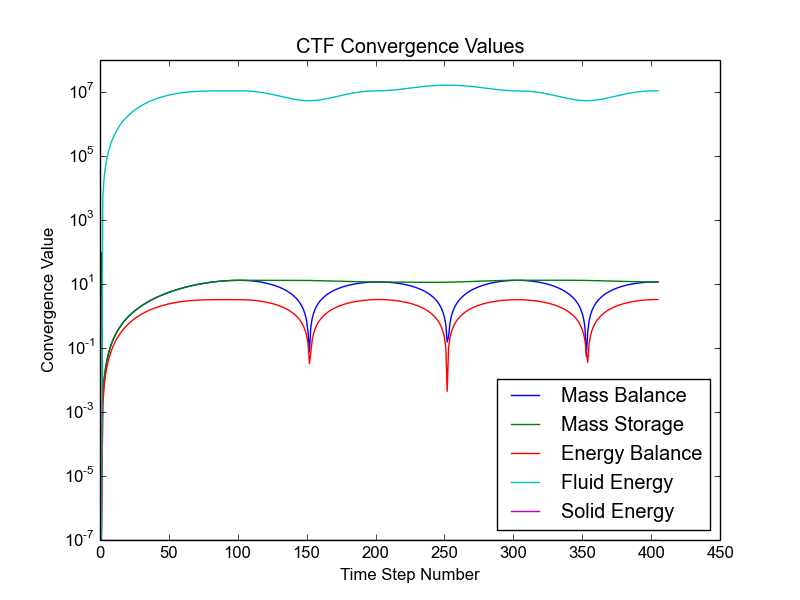
\includegraphics[width=0.50\textwidth]{images/Code_Verification/run_00_00/original/results/Convergence_Plot}
	\caption{Code Convergence Criteria for the Original Version of CTF}
	\label{fig:Code_Convergence:Original}
\end{figure}

\begin{figure}[!h]
	\centering
	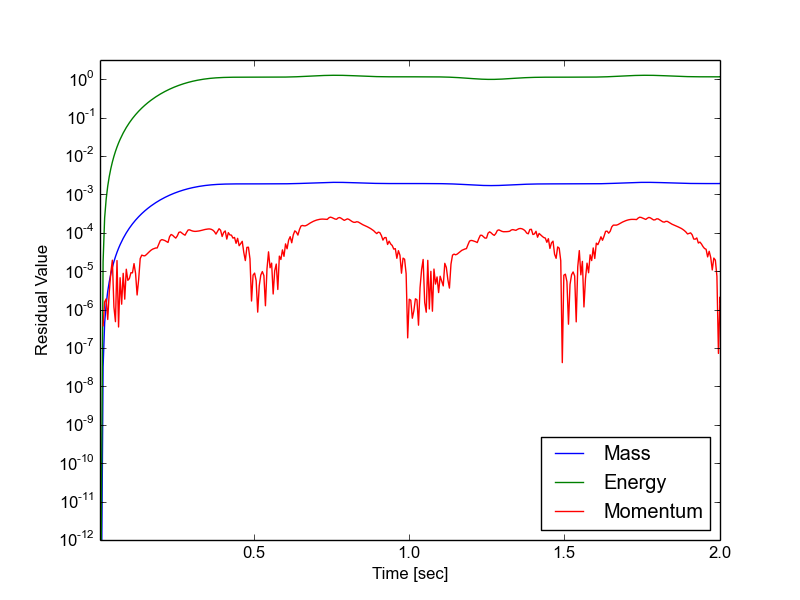
\includegraphics[width=0.50\textwidth]{images/Code_Verification/run_00_00/residual/results/Residuals_Plot}
	\caption{Summation of the Residuals for the Residual Version of CTF}
	\label{fig:Residuals_Plot}
\end{figure}

The residual formulation prints out the summation of the equation residuals
across the domain to an output file at the end of each time step and can be seen
in figure \ref{fig:Residuals_Plot}. The mass equation residual is in units of
$\frac{kg}{m^{3}s}$. The energy equation residual is in units of
$\frac{kW}{m^{3}}$. The momentum residual is in units of
$\frac{kg}{m^{2}s^{2}}$. The flat profile of the The residuals could have
expanded to provide convergence information at every position, variable, and equation. This would be
useful if any localized phenomenon was causing instabilities are numerical
error.

%\subsection{Error Quantification}
%
%\begin{figure}[!h]
%	\centering
%	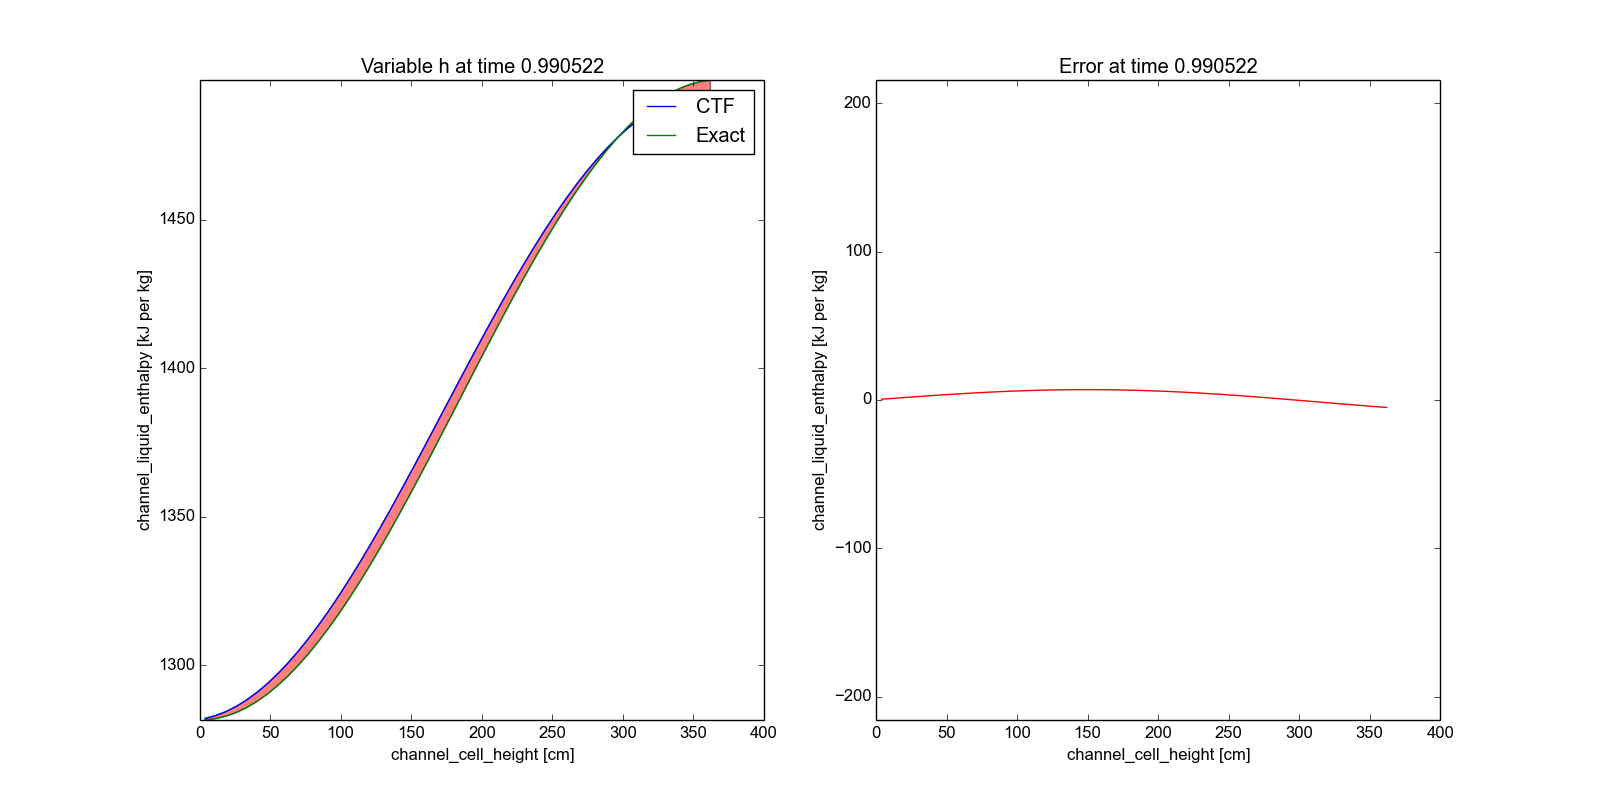
\includegraphics[width=1.00\textwidth]{images/Code_Verification/run_00_01/residual/results/tmp/h_0200.png}
%	\caption{Summation of the residuals for the residual version of CTF}
%	\label{fig:Residuals_Plot}
%\end{figure}
%
%\begin{figure}[!h]
%	\centering
%	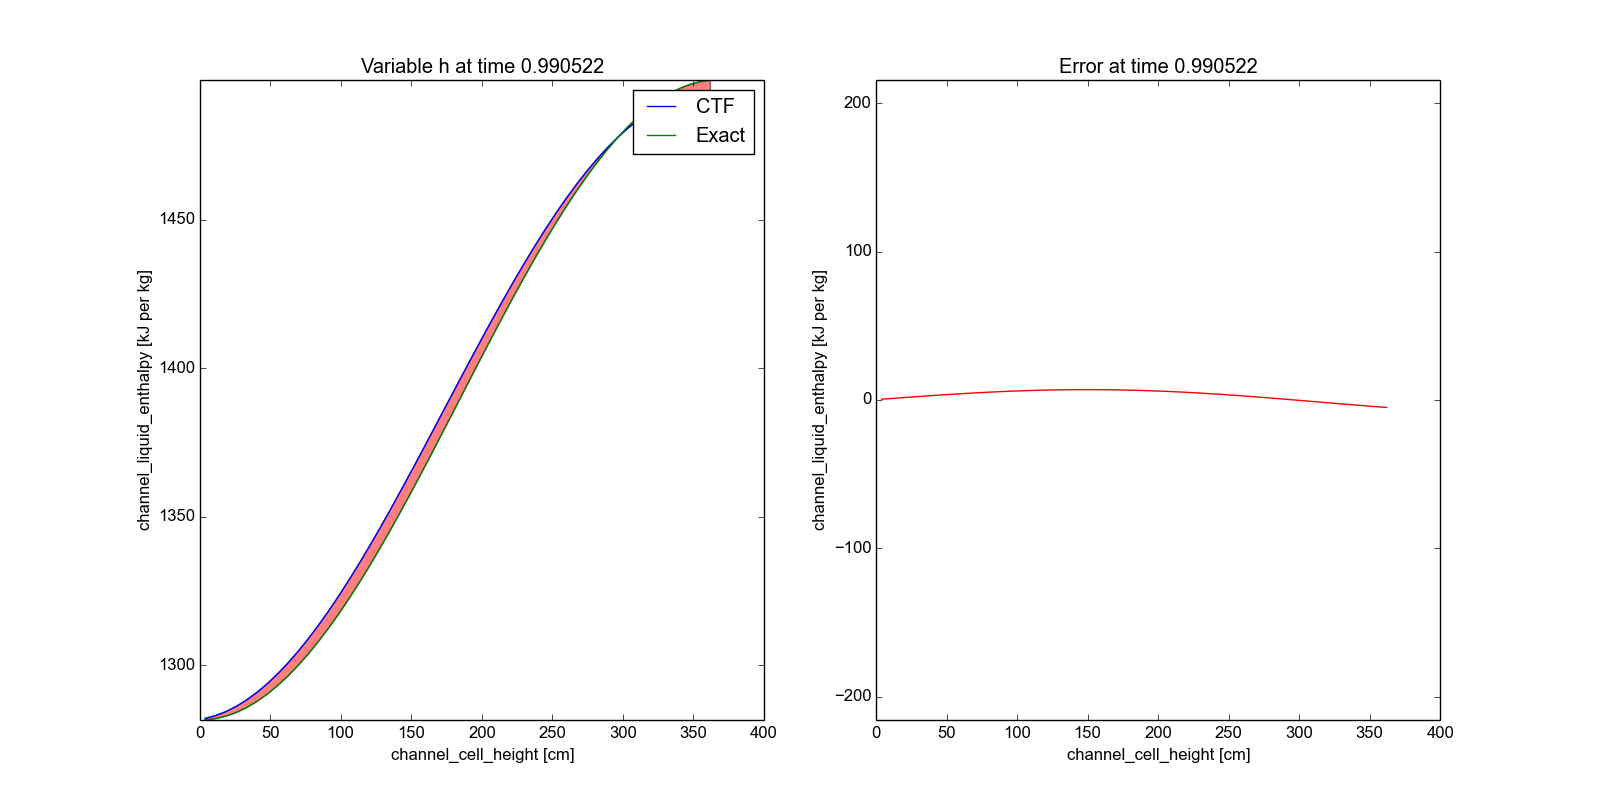
\includegraphics[width=0.55\textwidth]{images/Code_Verification/run_00_01/residual/results/tmp/h_0200}
%	\caption{Summation of the residuals for the residual version of CTF}
%	\label{fig:Residuals_Plot}
%\end{figure}

\subsection{Modified Equation Analysis}
    
    Because the velocity is constant, it can be pulled out of the spatial
    derivative as shown in equation \ref{eq:isokinetic_start}. Using upwinding,
    the finite difference can be written to look like equation
    \ref{eq:mass_isok_fd}. A second order Taylor series approximation can be
    used for $\rho_{i}^{n+1}$ and $\rho_{i-1}^{n}$ as shown in equations
    \ref{eq:rho_taylor_series_time} and \ref{eq:rho_taylor_series_space}
    respectively. The higher order terms ($O(\Delta x^{2},\Delta t^{2} )$) are
    not taken into account for this approximation. The Taylor series
    approximations can then be substituted into \ref{eq:mass_isok_fd} to yield
    \ref{eq:MEA_start}. This is the beginning of the modified equation analysis.
    The goal will be to isolate the original PDE and define the truncation error.
    
    \begin{equation}
    	\label{eq:isokinetic_start}
    	\frac{\partial \rho}{\partial t} + U_{0} \frac{\partial \rho}{\partial x} = 0
    \end{equation}
    
    \begin{equation}
    	\label{eq:mass_isok_fd}
    	\frac{ \rho_{i}^{n+1} - \rho_{i}^{n} }{\Delta t} 
    	+ U_{0} \frac{\rho_{i}^{n} - \rho_{i-1}^{n}}{\Delta x} = 0
    \end{equation}
    
    \begin{equation}
    	\label{eq:rho_taylor_series_time}
    	\rho_{i}^{n+1} =  \rho_{i}^{n} + 
    	\frac{\partial \rho}{\partial t} \Delta t +
    	\frac{1}{2} \frac{\partial^2 \rho}{\partial t^2} \Delta t^2 + O(\Delta t^{3})
    \end{equation}
    
    \begin{equation}
    	\label{eq:rho_taylor_series_space}
    	\rho_{i-1}^{n} =  \rho_{i}^{n} - 
    	\frac{\partial \rho}{\partial x} \Delta x +
    	\frac{1}{2} \frac{\partial^2 \rho}{\partial x^2} \Delta x^2 + O(\Delta x^{3})
    \end{equation}
    
    The lengthy equation \ref{eq:MEA_start} can be reduced to equation
    \ref{eq:MEA_p0} since the $\rho_{i}^{n}$ terms subtract out and the $\Delta
    t$ and $\Delta x$ terms in the denominator cancel out. This reduced equation
    can the be re-written into equation \ref{eq:MEA_p1}, with the original PDE
    followed by the truncation terms. 
    
    \begin{equation}
    	\label{eq:MEA_start}
    	\frac{ \left( \rho_{i}^{n} + \frac{\partial \rho}{\partial t} \Delta t +
    	\frac{1}{2} \frac{\partial^2 \rho}{\partial t^2} \Delta t^2 \right)-\rho_{i}^{n} }{\Delta t} 
    	+ U_{0} \frac{\rho_{i}^{n} - \left( \rho_{i}^{n} -  \frac{\partial \rho}{\partial x} \Delta x + 
    	\frac{1}{2} \frac{\partial^2 \rho}{\partial x^2} \Delta x^2 \right)}{\Delta x} 
    	+ O(\Delta x^{2},\Delta t^{2}) 
    	= 0
    \end{equation}
    
    \begin{equation}
    	\label{eq:MEA_p0}
    	 \frac{\partial \rho}{\partial t}  + \frac{1}{2} \frac{\partial^2 \rho}{\partial t^2} \Delta t +
    	 U_{0} \left(   \frac{\partial \rho}{\partial x}  - \frac{1}{2} \frac{\partial^2 \rho}{\partial x^2} \Delta x \right) 
    	 + O(\Delta x^{2},\Delta t^{2}) 
    	 = 0
    \end{equation}
    
    The terms to the right of the original PDE are the first order accurate
    truncation terms. Notice how the truncation error is  dependent on both the
    on the second derivatives of density with respect to space and time, and on
    the numerical spacing $\Delta t$ and $\Delta x$. Since the truncation
    error is linearly dependent on $\Delta t$ and $\Delta x$, the order of
    accuracy is 1 with respect to time and space. 
    
    \begin{equation}
    	\label{eq:MEA_p1}
    	 \frac{\partial \rho}{\partial t}  +  U_{0} \frac{\partial \rho}{\partial x} + 
    	 \frac{1}{2} \frac{\partial^2 \rho}{\partial t^2} \Delta t -
    	   U_{0}  \frac{1}{2} \frac{\partial^2 \rho}{\partial x^2} \Delta x  
    	   + O(\Delta x^{2},\Delta t^{2}) = 0 
    \end{equation} 
    
    When the energy equation undergoes a similar modified eqution analysis, the
    order of accuracy is also 1 for time and space. The momentum conservation
    equation does not apply for this problem since the velocity is
    constant.
    
%    Before we can procede, we need to take the derivative of the original PDE with respect
%    to space and time as shown in equations \ref{eq:mass_dt} and  \ref{eq:mass_dx} 
%    respectively. These two derivatives can substitute into each other using the common 
%    term $\frac{\partial^2 \rho}{\partial x \partial t}$. The second derivatives of density with 
%    respect to space and time are therefore related by the velocity squared as
%    shown by equation \ref{eq:mass_second_derivatives}.
%    
%    \begin{equation}
%    \label{eq:mass_dt}
%    	 \frac{\partial^2 \rho}{\partial t^2} + U_{0} \frac{\partial^2 \rho}{\partial x \partial t} = 0
%    \end{equation}
%    
%    \begin{equation}
%    \label{eq:mass_dx}
%    	 \frac{\partial^2 \rho}{\partial t \partial x} + U_{0} \frac{\partial^2 \rho}{\partial x^2} = 0
%    \end{equation}
%    
%    \begin{equation}
%    \label{eq:mass_second_derivatives}
%    	 \frac{\partial^2 \rho}{\partial t^2} =  U_{0}^2 \frac{\partial^2 \rho}{\partial x^2}
%    \end{equation} \linebreak
%    
%    This relationship can then be substituted back into equation \ref{eq:MEA_p1}, 
%    which can be reduced to equation \ref{eq:MEA_result} after igonoring the higher
%    order terms. The error depends on the CFL number, the axial spacing, and the
%    second order derivative of density with respect to space. This derivative is
%    what gives the error the characterisitcs of diffusion. When the CFL number is
%    less than one, the error term is negative and the diffusion is dampening. When
%    the CFL number is greater than one, the error term becomes positive, and the
%    accumulation of the error destabilizes the solution. 
%    
%    \begin{equation}
%    	 \frac{\partial \rho}{\partial t}  +  U_{0} \frac{\partial \rho}{\partial x} - 
%    	  \frac{1}{2}  \left(  \Delta x U_{0} \frac{\partial^2 \rho}{\partial
%    	  x^2} -   U_{0}^2 \frac{\partial^2 \rho}{\partial x^2} \Delta t  \right) 
%    	   + O(\Delta x^{2},\Delta t^{2}) = 0
%    \end{equation}
%    
%    \begin{equation}
%    \label{eq:MEA_result}
%    	 \frac{\partial \rho}{\partial t}  +  U_{0} \frac{\partial \rho}{\partial x} - 
%    	 \frac{\Delta x U_{0}}{2} \frac{\partial^2 \rho}{\partial x^2}  
%    	 \left(  1 - CFL  \right) 
%    	 + O(\Delta x^{2},\Delta t^{2})  = 0
%    \end{equation}
%    
%    Modified eqauation analysis can be applied to the energy balance equation
%    presented in equation \ref{eq:MEA_energy}. The energy equation is presented in a form where
%    the momentum equation was substituted in as zero and then divided through by
%    density. The result presented in equation \ref{eq:MEA_ene_result} is similar in
%    form to the result for the mass balance equation \ref{eq:MEA_result}.
%    
%    \begin{equation}
%    	\label{eq:MEA_energy}
%    	\frac{\partial h}{\partial t} - \frac{1}{\rho} \frac{\partial P}{\partial t} +
%    	U_{0} \frac{\partial h}{\partial x} = 0
%    \end{equation}
%    
%    \begin{equation}
%    \label{eq:MEA_ene_result}
%    	\frac{\partial h}{\partial t} - \frac{1}{\rho} \frac{\partial P}{\partial t} +
%    	U_{0} \frac{\partial h}{\partial x} - 
%    	\frac{\Delta x U_{0}}{2} \frac{\partial^2 h}{\partial x^2}
%    	\left( 1 - CFL \right)
%    	= 0
%    \end{equation}

\section{Richardson Extrapolation}

The Richardson extrapolation was performed by refining the spatial and temporal
step sizes by a factor of 2 for a set number of times. The spatial and temporal
studies are refined separately in their own study in order to isolate the
spatial and temporal affects on the solution. The generation of the inputs,
running of the codes, and analysis of the output were automated with a python
script in order to reduce user input errors and increase repeatability.  For
this analysis, a significant amount of information was added to the hdf5 output
files, increasing memory usage and run time. The computational resources for the
spatial study was much higher than the temporal study due to the need to keep
the courant number below 0.500. To keep the computational resources needed
to perform this analysis reasonable, fewer spatial refinements were performed
compared to the temporal analysis.

\subsection{Convergence of Error}

The relative difference at each point for a particular time step was calculated
between each iteration for each quantity of interest. For the spatial
refinement, the lower iterate values were numerically integrated to match the
shape of the initial domain. The errors were then summed over the entire domain
to yield a total error for each variable. The total error for density is
plotted in figures \ref{fig:Temporal:Diff_rho} and \ref{fig:Spatial:Diff_rho} as
a function of temporal and spatial step size. 

\begin{figure}[!h]
	\centering
	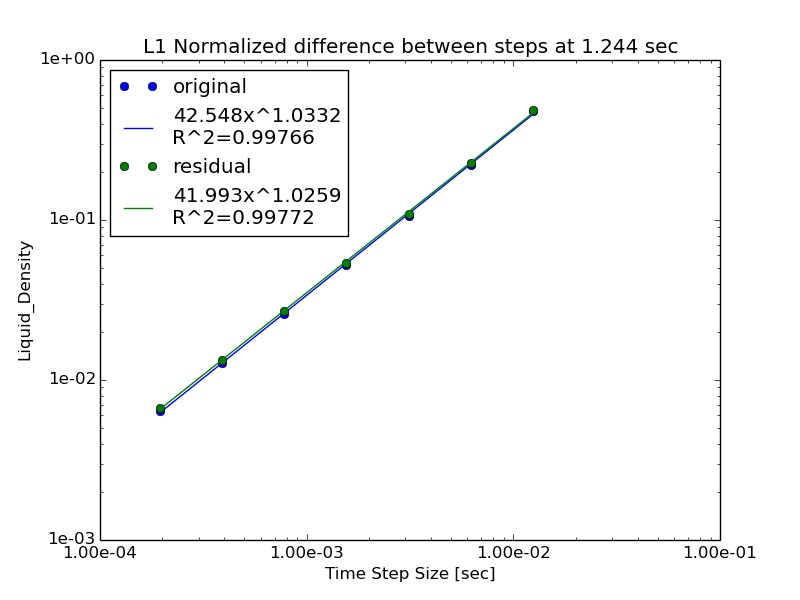
\includegraphics[width=0.55\textwidth]{images/Temporal_Study/Difference_rho}
	\caption{Difference Between Successive Temporal Refinements for Density}
	\label{fig:Temporal:Diff_rho}
\end{figure} 

The data points were chosen to be inside of the asymptotic range as shown by
the good power fit with an exponent near 1. The power fit shows that as the
temporal and spatial step sizes are reduced, the numerical error approaches
zero. The discretization error between the original version of CTF is
relatively small and is most likely due to the small fluctuations in the
velocity present in the original version of the code. 

\begin{figure}[!h]
	\centering
	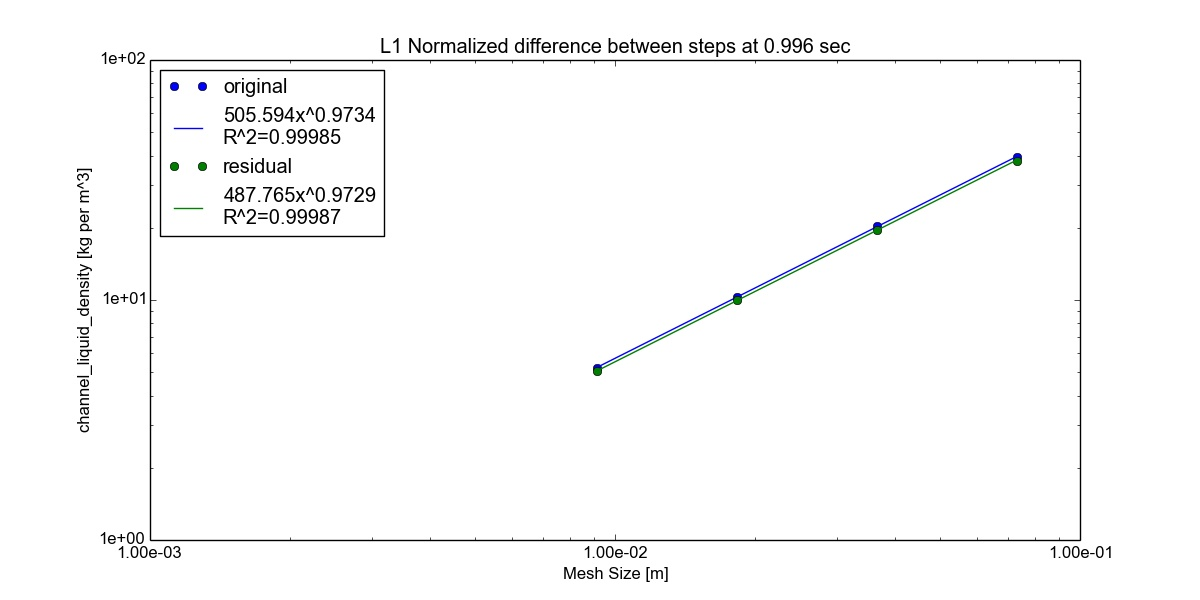
\includegraphics[width=0.55\textwidth]{images/Spatial_Study/Difference_rho}
	\caption{Difference Between Successive Spatial Refinements for Density}
	\label{fig:Spatial:Diff_rho}
\end{figure} 

\subsection{Order of Accuracy}

The order of accuracy for this verification problem is first order as shown by
the modified equation analysis. This can be considered to be the exponent on
the power fits as seen in figures \ref{fig:Temporal:Diff_rho}. However the order
of accuracy $p$ can be calculated by using equation \ref{eq:OOA} where $f_{1}$,
$f_{2}$, $f_{3}$ are consecutive levels within the same Richardson extrapolation
study. The refinement factor, $R$, has the constant value of 2 for both the
spatial and temporal studies.

\begin{equation}
	\label{eq:OOA}
	p= \frac{
	      	ln \left(
	      	\frac{f_{3}-f_{2}}{f_{2}-f_{1}}
	      	\right)
	    }{ln(R)}
\end{equation}

The order of accuracy for all of the variables are presented for the temporal
analysis and spatial analysis in figures \ref{fig:Temporal:OOA} and
\ref{fig:Spatial:OOA} respectively. The temporal order of accuracy is well
within the asymptotic range for the whole analysis, and moves closer to 1.0 with
decreasing time step size. The spatial order of accuracy is a slightly outside
the asymptotic range, but approaches an order of accuracy of 1.0 with
decreasing mesh size. 

\begin{figure}[!h]
	\centering
	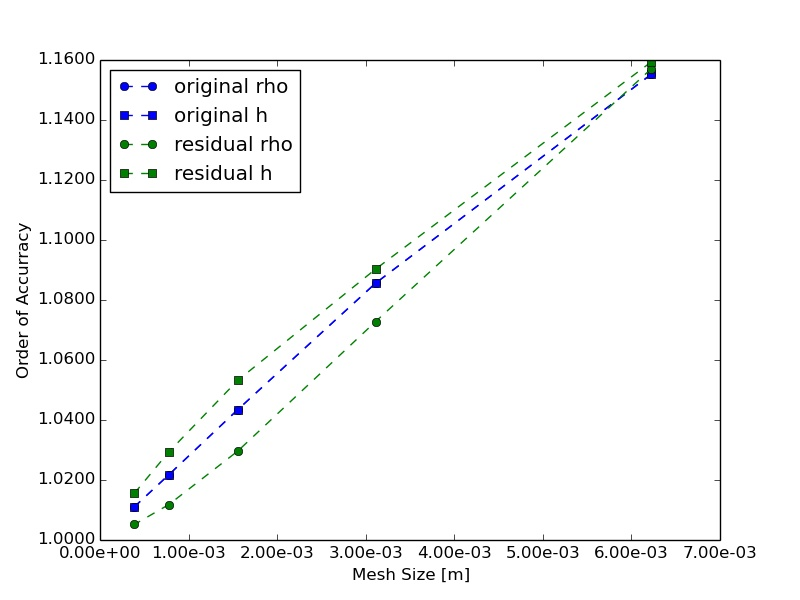
\includegraphics[width=0.55\textwidth]{images/Temporal_Study/Order_Of_Accuracy_Summary}
	\caption{Temporal Order of Accuracy}
	\label{fig:Temporal:OOA}
\end{figure}

The slight differences between the original version of CTF and the residual
formulation might be due to the different solution methods and back substitution
of variables. Despite the small differences, both versions of the code exhibit
order of accuracies very close the values obtained through the modified
equation analysis.

\begin{figure}[!h]
	\centering
	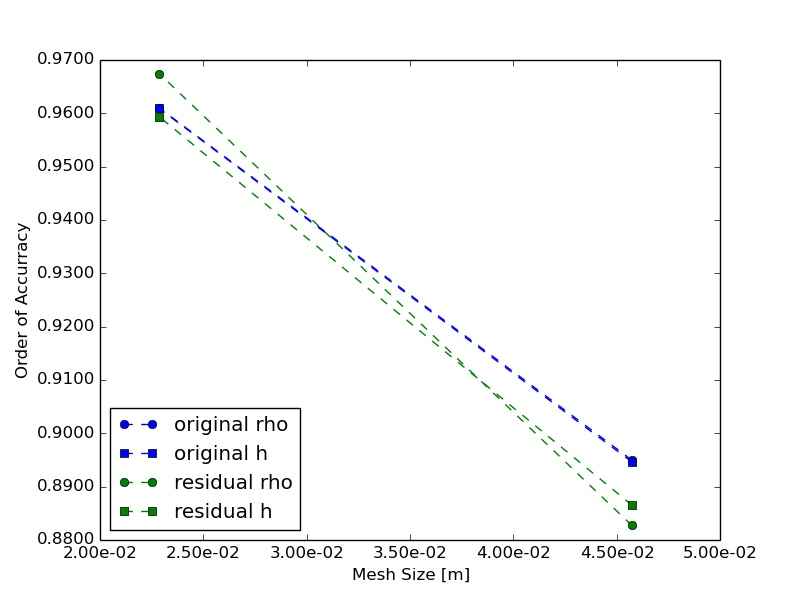
\includegraphics[width=0.55\textwidth]{images/Spatial_Study/Order_Of_Accuracy_Summary}
	\caption{Spatial Order of Accuracy}
	\label{fig:Spatial:OOA}
\end{figure}

%\section{Parameter Study}
%
%Tables and figures of varying the results.
%
%\subsection{Changes in $\Delta$T}
%
%This changes the amplitude of the displacement
%
%\subsection{Changes in frequency}
%
%This changes the frequency of the displacement
%
%\subsection{Changes in Mass Flow Rate}
%
%\section{Computational Time}
%
%The computational time of the two methods for different computational sizes.
%Compare the semi-implicit and fully implicit methods at 0.5 , 1.0, and 2.0 CFL. 

\section{Conclusions}

The residual formulation of CTF allows for a numerical computation of the
multivariable Jacobian matrix compared to the original analytical derivation of
a pressure matrix. The 1-D isokinetic single phase liquid verification problem
is a good verification problem through its isolation of the order
of accuracies through modified equation analysis. The discretization error for
both versions of the code converged to zero with decreasing time step and axial
mesh size. The order of accuracy for the temporal and spatial refinements
matched very closely with the modified equation analysis for both codes. For all
of these data points, the residual formulation of the code showed discretization
errors that were very close with the original version of the code. Future work
might be comparing the numerical error obtained in the code to the analytical
error predicted by the modified equation analysis using the derivatives of the
known solutions. While within the assymptotic range, the first order accurate
analytical error should almost exactly match the error from the code.

%%%%%%%%%%%%%%%%%%%%%%%%%%%%%%%%%%%%%%%%%%%%%%%%%%%%%%%%%%%%%%%%%%%%%
\section{Acknowledgments}

Dr. Kostadin Ivanov and everyone in the RDFMG

%%%%%%%%%%%%%%%%%%%%%%%%%%%%%%%%%%%%%%%%%%%%%%%%%%%%%%%%%%%%%%%%%%%%%
\setlength{\baselineskip}{12pt}

\bibliographystyle{mc2015}
\bibliography{references}

%%%%%%%%%%%%%%%%%%%%%%%%%%%%%%%%%%%%%%%%%%%%%%%%%%%%%%%%%%%%%%%%%%%%%

%\appendix
%\section{}


\end{document}
